\clearpage
\section{Quy trình chạy và trình bày demo}
\subsection{Chuẩn bị môi trường và tài nguyên trước khi quay}
Mỗi terminal cần source cùng workspace và môi trường Python để ROS, cv\_bridge và torch tương thích. Môi trường ảo bật system-site-packages cho thư viện ROS; script bổ sung site-packages vì executable ROS có thể dùng shebang Python hệ thống. Giới hạn thread CPU giúp giảm cạnh tranh tài nguyên với simulator.
\begin{lstlisting}[language=bash,caption={Chuẩn bị workspace và tài nguyên trước lượt demo},label={lst:prepare}]
cd ~/turtlebot4_lab_ws
source /opt/ros/humble/setup.bash
colcon build --symlink-install --packages-select turtlebot4_lab05
source lab_env.bash
source src/turtlebot4_lab05/scripts/lab05_env.bash
python src/turtlebot4_lab05/scripts/download_resources.py \
  --cache "$TB4_LAB05_CACHE"
python src/turtlebot4_lab05/scripts/check_scene.py
\end{lstlisting}
Các lệnh tiếp theo chạy ở terminal riêng, đều bắt đầu bằng \code{cd ~/turtlebot4_lab_ws}, source \code{lab_env.bash} và \code{lab05_env.bash} như trên. Không mở hai simulator cùng partition hoặc hai bộ Nav2 trùng namespace.
\begin{lstlisting}[language=bash,caption={Terminal A và C: simulator, vật thể và undock},label={lst:sim}]
# Terminal A: keep running
ros2 launch turtlebot4_lab simulation.launch.py \
  model:=standard rviz:=false

# Terminal C: after simulator is ready
ros2 run turtlebot4_lab05 spawn_demo_objects
ros2 action send_goal /undock \
  irobot_create_msgs/action/Undock '{}' --feedback
\end{lstlisting}
Chờ undock SUCCEEDED. Với world mới chỉ spawn một lần. Nếu đã có scene cũ, dùng \code{spawn_demo_objects --ros-args -p replace_existing:=true} thay lệnh spawn thường, trước khi bắt đầu mission. Nó chỉ thay các tên model lab05 được cấu hình và retired; không sửa tường/nền/robot.

\subsection{Bắt đầu quay khi nạp map và đặt initial pose}
Bấm Record \textbf{trước} khi chạy Terminal B để thấy quá trình nạp lại bản đồ. Sắp xếp RViz, camera và terminal mission sao cho đọc được kết quả mà vẫn thấy robot di chuyển.
\begin{lstlisting}[language=bash,caption={Terminal B: nạp map cũ, AMCL và Nav2},label={lst:bringup}]
ros2 launch turtlebot4_lab05 bringup.launch.py \
  start_yolo:=false start_navigation:=false
\end{lstlisting}
RViz phải có Fixed Frame map, Map, LiDAR scan, AMCL pose và costmap. Thao tác 2D Pose Estimate như phần định vị; đối chiếu scan với tường. Nếu dùng helper ground truth trước mission, thuyết minh rõ nguồn initial pose. Chưa bật mission khi localization còn sai.
\clearpage

\subsection{Chạy YOLO và chuỗi ba goal khi đang quay}
\begin{lstlisting}[language=bash,caption={Terminal D, E, F: nhận diện, observer và mission},label={lst:mission}]
# Terminal D: real camera + YOLO window
ros2 launch turtlebot4_lab05 yolo.launch.py \
  device:=0 show_window:=true

# Terminal E: passive observer (optional, before mission)
python src/turtlebot4_lab05/scripts/record_demo.py \
  --output-directory "$TB4_LAB_WS/log/video_evidence"

# Terminal F: only after localization has been checked
export LAB05_VIDEO_LOG="$TB4_LAB_WS/log/navigation_video.jsonl"
ros2 run turtlebot4_lab05 sequential_navigation --ros-args \
  --params-file src/turtlebot4_lab05/config/navigation.yaml \
  -p localization_confirmed:=true \
  -p log_file:="$LAB05_VIDEO_LOG"
\end{lstlisting}
Dùng thư mục/tên log mới cho mỗi lượt quay để tránh trộn nhiều mission. Khi chạy F, không teleop, không bấm Nav2 Goal và không cập nhật initial pose giữa đường. Code sẽ tự gửi Goal\_1, dừng 8 s sau thành công, rồi Goal\_2 và Goal\_3; không cần bấm Enter ở mỗi goal.
\begin{table}[H]\centering\small
\caption{Các mốc phải xuất hiện trong video}
\begin{tabularx}{\linewidth}{@{}P{3.8cm}Y@{}}\toprule
Mốc&Nội dung cần nhìn thấy/giải thích\\\midrule
Nạp map&Lệnh bringup, map cũ trên RViz, localization active.\\
Đặt pose&2D Pose Estimate hoặc helper được nói rõ; scan khớp map.\\
Bắt đầu mission&readiness\_passed, goal\_accepted; đường trên RViz và camera đang cập nhật.\\
Chuyển goal tự động&goal\_result status=4 của Goal\_1 rồi Goal\_2; code tự chuyển sau dwell.\\
Kết thúc&Goal\_3 status=4; mission\_completed completed=3; camera vẫn mở; robot dừng.\\\bottomrule
\end{tabularx}\end{table}
Giữ quay liên tục quá trình di chuyển và camera, rồi quay thêm 5--10 s bảng kết quả cuối. Không chỉ quay terminal in ba dòng SUCCEEDED vì chưa chứng minh robot đã thực hiện đường đi và YOLO hoạt động song song. Kịch bản chi tiết từng terminal nằm trong \code{VIDEO_DEMO.md}.

\subsection{Quan sát và ghi bằng chứng}
\code{record_demo.py} chỉ subscribe, không phát goal/vận tốc. Observer đối chiếu stamp/frame id ảnh annotated với RGB, đếm inference trong khi odometry có $|v_x|>0.02$ m/s hoặc $|\omega_z|>0.05$ rad/s; lưu action status, AMCL, ground truth, plan và hazard. Chỉ số này chứng minh xử lý ảnh khi có chuyển động theo ngưỡng, không tự chứng minh nhãn của mọi frame đều đúng.
\clearpage

\section{Kết quả thực nghiệm và hình ảnh minh họa}
\subsection{Ảnh trích trực tiếp từ video demo đã cung cấp}
\begin{figure}[H]\centering
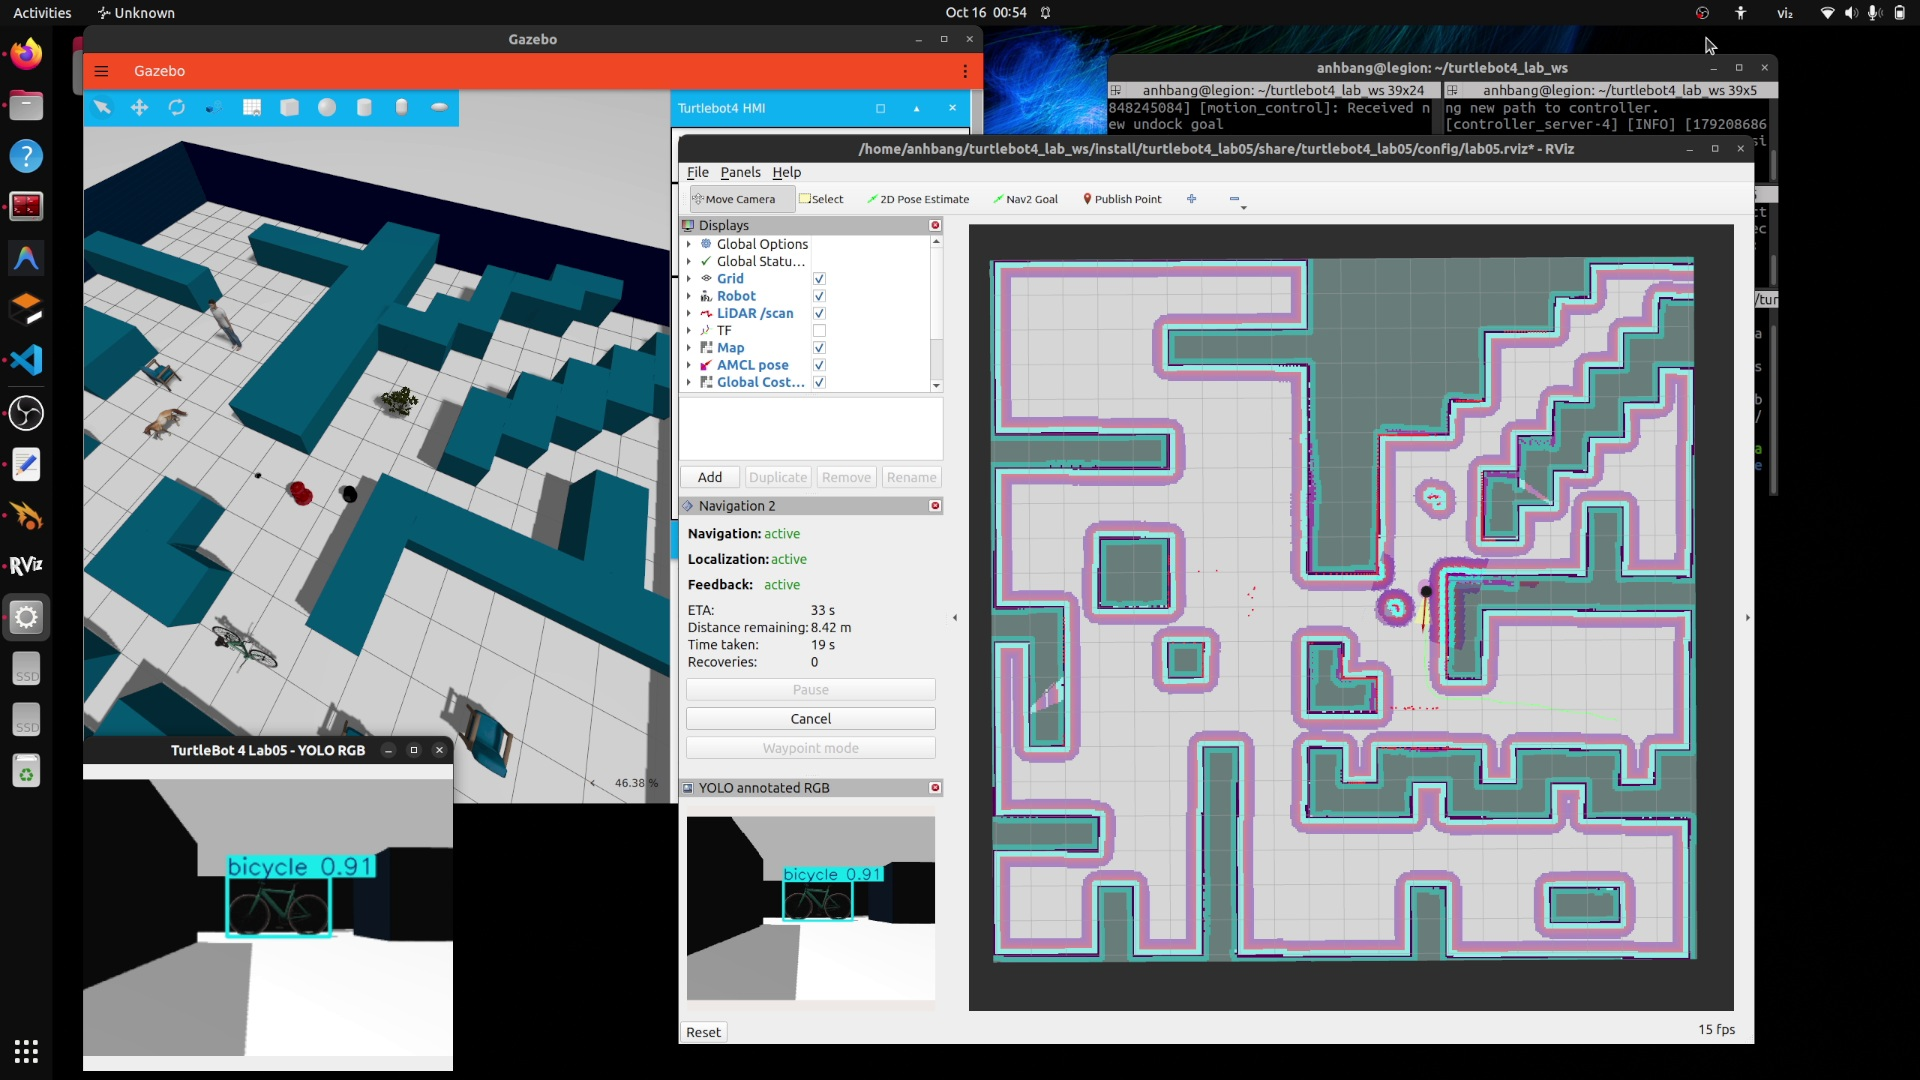
\includegraphics[width=\linewidth]{figures/video_navigation.jpg}
\caption[Video: RViz và YOLO hoạt động đồng thời]{Khung hình tại 08:04.7 của video Drive: simulator có xe đạp và trụ cứu hỏa, RViz báo Navigation/Localization/Feedback active, còn 8.42 m và recovery 0; cửa sổ YOLO nhận bicycle 0.91 cùng lúc. Đây là ảnh trích video thật, không phải lần chạy mới do quá trình rà soát tạo ra.}\label{fig:videoactive}
\end{figure}
\begin{figure}[H]\centering
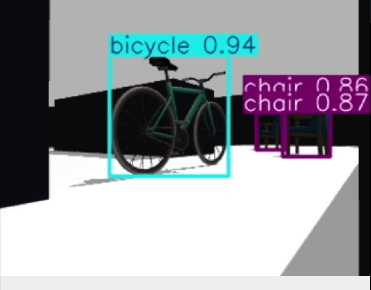
\includegraphics[width=.49\linewidth,height=5.1cm,keepaspectratio]{figures/video_bicycle.jpg}
\caption[Video: xe đạp và ghế được YOLO nhận diện]{Crop cửa sổ camera ở 15:49.9: bicycle 0.94 và chair 0.86/0.87. Crop chỉ bỏ phần desktop xung quanh; bbox và nhãn giữ nguyên từ video.}\label{fig:videobicycle}
\end{figure}
Video dài khoảng 16 phút 09 giây, độ phân giải $1920\times1080$, 60 FPS của bản ghi màn hình. FPS video không phải FPS camera hay inference. Thời điểm trên là vị trí trong tệp, không phải simulation time. Các khung trích xác nhận hình ảnh phiên bản có xe đạp và cửa sổ nhận diện; các bảng số liệu ở phần sau vẫn dùng log đúng lượt và phiên bản đã ghi.
\clearpage

\subsection{Nạp map, localization và đường đi trên RViz2}
\begin{figure}[H]\centering
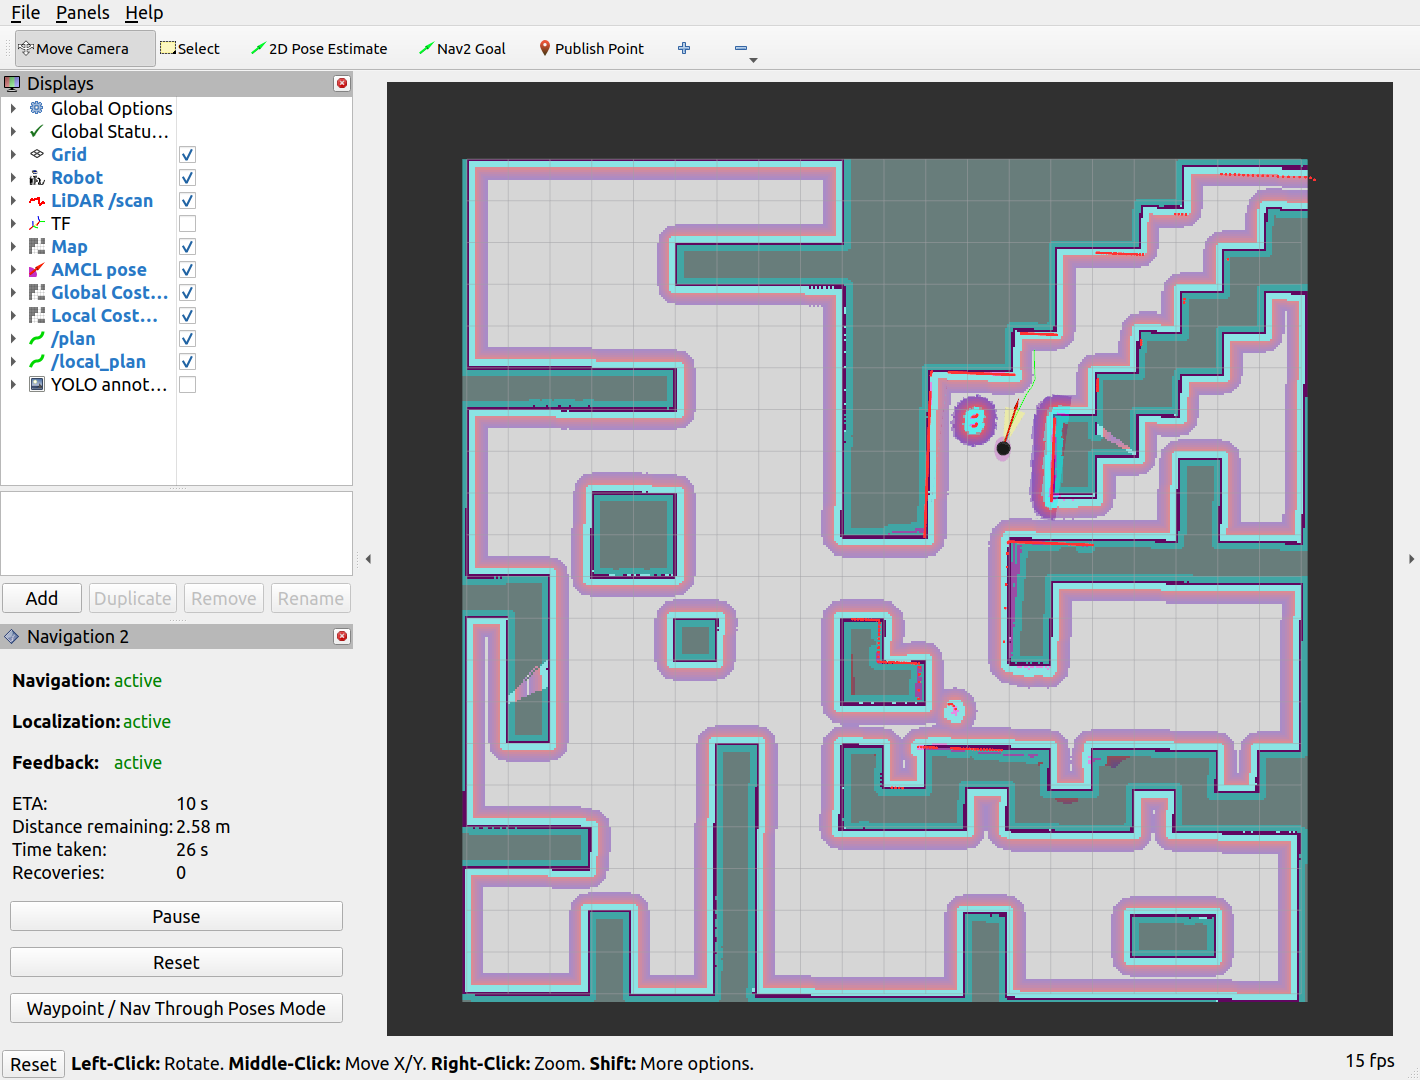
\includegraphics[width=\linewidth,height=14.1cm,keepaspectratio]{figures/rviz_navigation.png}
\caption[Map, localization và đường đi trên RViz]{Ảnh RViz native của lượt đã lưu ngày 15/10/2026: Localization và Navigation active; scan, costmap, robot và path trong lúc Goal\_3 đang chạy. Feedback còn 2.58 m, recovery 0 tại thời điểm chụp. Scene của ảnh thuộc phiên bản lịch sử sáu vật thể.}\label{fig:rviz}
\end{figure}
Ảnh cho thấy map đang được dùng với LiDAR và costmap; không phải map mới tạo bởi SLAM. Đường toàn cục là hướng di chuyển qua không gian có chi phí thấp, đường cục bộ là quỹ đạo ngắn từ DWB. Feedback trên ảnh là tiến độ tại thời điểm chụp, chưa phải chứng cứ SUCCEEDED; kết quả action sau đó được đối chiếu bằng UUID và log.

Nguồn ảnh: \code{validation/scattered_rviz_during_navigation.png}. Tệp \code{scattered_windows_during_navigation.json} ghi thời điểm native window đang hiển thị và trạng thái mission RUNNING; ảnh màn hình không được dựng lại bằng đồ họa để thay kết quả thực nghiệm.
\clearpage

\subsection{Ba goal liên tiếp và quỹ đạo thực đo}
\begin{figure}[H]\centering
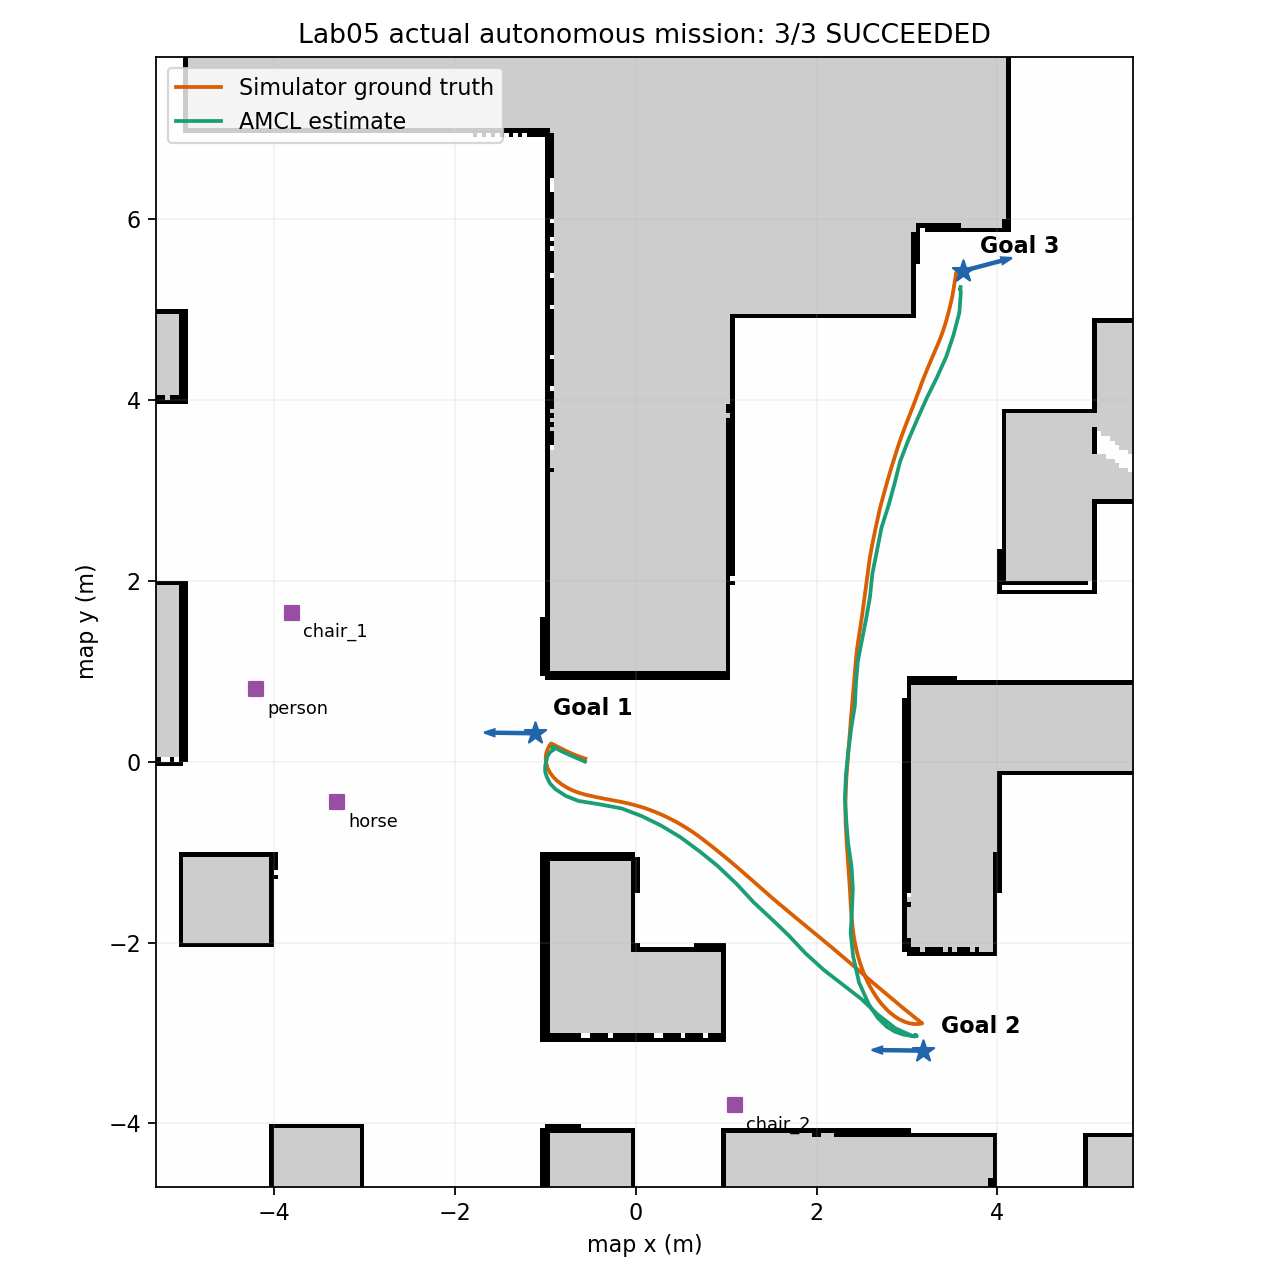
\includegraphics[width=.88\linewidth,height=12.0cm,keepaspectratio]{figures/trajectory_historical.png}
\caption[Quỹ đạo AMCL và ground truth của lượt baseline]{Quỹ đạo ground truth và AMCL của lượt baseline đã lưu ngày 15/10/2026. Sao và mũi tên chỉ goal/yaw; các marker tím là vật thể của scene bốn vật thể cũ, không phải bố trí tám vật thể hiện tại. Đây là quỹ đạo quan sát được, không phải đường nội suy giữa goal.}\label{fig:trajectory}
\end{figure}
\begin{table}[H]\centering\small
\caption{Kết quả baseline và sai số vị trí gần thời điểm action kết thúc}\label{tab:errors}
\begin{tabular}{@{}lcrrr@{}}\toprule
Goal&Status&Sai số AMCL (m)&Sai số truth (m)&$|\Delta t|$ (s)\\\midrule
Goal\_1&SUCCEEDED (4)&0.246&0.211&0.138\\
Goal\_2&SUCCEEDED (4)&0.174&0.302&0.143\\
Goal\_3&SUCCEEDED (4)&0.178&0.073&0.081\\\bottomrule
\end{tabular}\end{table}
Sai số được tính $e=\sqrt{(x-x_g)^2+(y-y_g)^2}$ từ sample gần lúc action result, không phải phép đo chính xác tại thời điểm controller quyết định. Số liệu từ \code{demo_metrics.json}; chênh lệch truth/AMCL giải thích vì sao một action SUCCEEDED có thể đi kèm sai số truth lớn hơn xy tolerance.
\clearpage

\subsection{Nhận diện thực tế và bằng chứng chạy đồng thời}
\begin{figure}[H]\centering
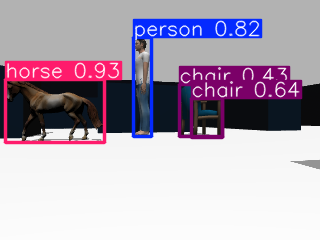
\includegraphics[width=.72\linewidth,height=5.4cm,keepaspectratio]{figures/yolo_observed.png}
\caption[Kết quả nhận diện person, horse và chair]{Ảnh RGB annotated thực tế ở lượt baseline: person 0.82, horse 0.93 và hai bbox chair. Ảnh gốc $320\times240$, được phóng to trong báo cáo; đây là ảnh của phiên bản YOLO lịch sử, không phải phép đo YOLO11s mới.}\label{fig:yoloactual}
\end{figure}
\begin{figure}[H]\centering
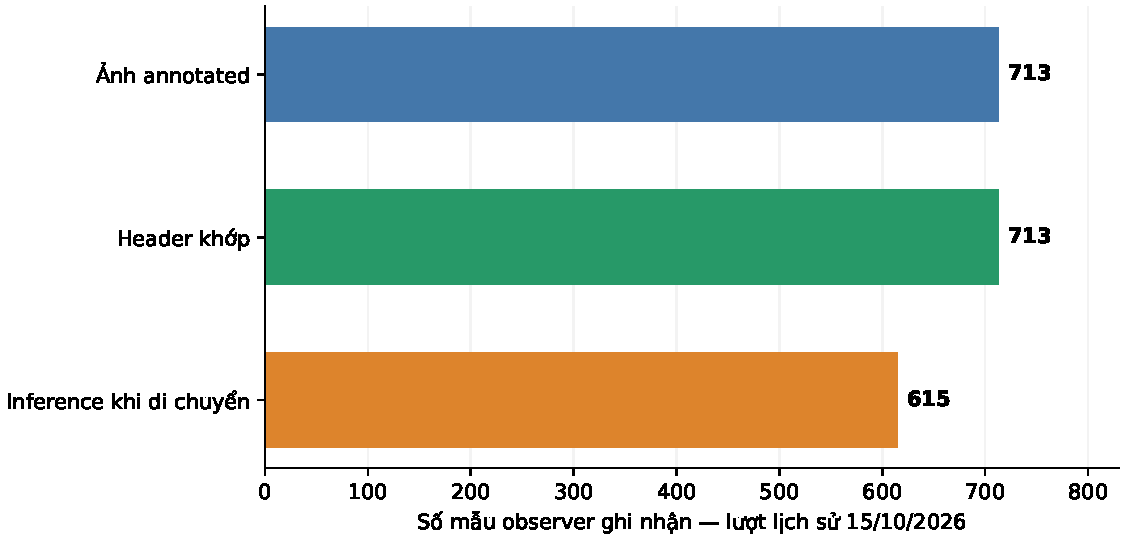
\includegraphics[width=.94\linewidth,height=3.3cm,keepaspectratio]{figures/parallel_evidence.pdf}
\caption[Số liệu nhận diện khi robot di chuyển]{Bằng chứng xử lý ảnh trong lượt sáu vật thể ngày 15/10/2026. Các số đếm lấy trực tiếp từ scattered\_demo\_summary.json.}\label{fig:parallel}
\end{figure}
\begin{table}[H]\centering\small
\caption{Tóm tắt lượt sáu vật thể đã lưu log}\label{tab:historical}
\begin{tabularx}{\linewidth}{@{}P{5.7cm}Y@{}}\toprule
Chỉ số&Kết quả quan sát\\\midrule
Action/mission&3/3 status=4; completed=3; yolo\_interrupted=false\\
RGB / annotated / header khớp&2561 / 713 / 713\\
Inference khi robot chuyển động&615; model thực ở cuda:0\\
Confidence lớn nhất đúng nhóm&person 0.925; horse 0.953; chair 0.895\\
Nhầm nhãn có trong log&dog 0.669; suitcase 0.624 (balô cũ); không tính là vật thể được nhận diện đúng\\
Hazard&Không ghi nhận bump, cliff, stall, wheel drop; có type 0 (backup limit)\\\bottomrule
\end{tabularx}\end{table}
Các confidence trong ảnh và bảng là từng prediction hoặc giá trị lớn nhất, không phải precision/recall/mAP. Lượt baseline riêng có median inference 116.13 ms, p95 156.55 ms, thời gian mission 162.34 s thực / 81.801 s mô phỏng (RTF khoảng 0.50). Các số này thuộc YOLO cũ; không dùng làm benchmark tốc độ YOLO11s với bộ lọc hiện tại.
